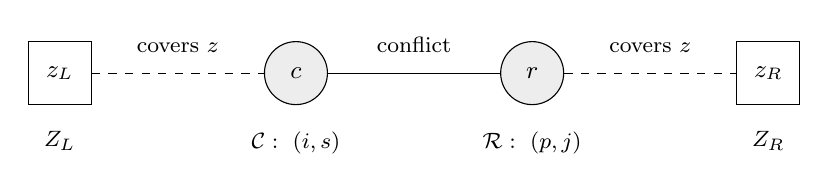
\begin{tikzpicture}[
  every node/.style={font=\small},
  original/.style={circle,draw,fill=black!7,minimum size=8mm,inner sep=1pt},
  copy/.style={rectangle,draw,minimum size=8mm,inner sep=3pt},
  edge label/.style={font=\footnotesize,above=4pt},
  family label/.style={font=\footnotesize,below=6pt}
]
 \node[copy] (zl) at (0,0) {$z_L$};
 \node[original] (c) at (3,0) {$c$};
 \node[original] (r) at (6,0) {$r$};
 \node[copy] (zr) at (9,0) {$z_R$};
 \draw[dashed] (zl) -- node[edge label] {covers $z$} (c);
 \draw (c) -- node[edge label] {conflict} (r);
 \draw[dashed] (r) -- node[edge label] {covers $z$} (zr);
 \node[family label] at (zl.south) {$Z_L$};
 \node[family label] at (c.south) {$\mathcal C:\ (i,s)$};
 \node[family label] at (r.south) {$\mathcal R:\ (p,j)$};
 \node[family label] at (zr.south) {$Z_R$};
\end{tikzpicture}
